% Predicting human metagame adaptation in a collectible card game.
% IEEE Transactions on Games / CoG submission draft.
%
% All numbers copied from committed experiment artifacts in
% classic_sim/examples/validation/README.md (sections S1-S4).
% Bibliography verified 2026-08-11 against publisher pages (DOIs included).
% TODO before submission:
%   - author block / affiliation / funding;
%   - decide venue (ToG regular paper vs CoG) and trim to page budget.

\documentclass[conference]{IEEEtran}
\usepackage{booktabs}
\usepackage{graphicx}
\usepackage{amsmath}
\usepackage{url}
\usepackage{tikz}
\usetikzlibrary{positioning,arrows.meta,calc}
\usepackage{pgfplots}
\pgfplotsset{compat=1.18}

\newcommand{\pp}{\,\text{pp}}

\begin{document}

\title{Predicting Human Metagame Adaptation to Expansions and Balance
Patches in a Collectible Card Game}

\author{\IEEEauthorblockN{Alex Elton-Pym}
\IEEEauthorblockA{\textit{(affiliation TODO)}\\
alexeltonpym@gmail.com}}

\maketitle

\begin{abstract}
Expansions and balance patches change which cards a population of
players puts in its decks. We test whether this response can be
predicted from simulation before it happens. The inputs are a
card-accurate simulator of 2014-era \emph{Hearthstone} and the real
decks played before each of two historical shocks, the Naxxramas
expansion (July 2014) and the Starving Buzzard nerf (September 2014);
ground truth for the outcome comes from 33{,}697 ranked decklists.
Unbiased evolutionary deck search adopts new cards at roughly the
mutation-drift rate, because a single card changes a 30-card deck's
win rate by about 1$\pp$ while affordable per-deck evaluation is an
order of magnitude noisier. We instead measure each candidate card's
marginal win-rate contribution in fixed real host decks. This probe
recovers the community's adoption ranking of the new set, and
evolution whose mutation operator is weighted by probed values, as a
model of players' deliberate testing of promising cards, reproduces
the post-shock decklists on the cards that moved. Direction hit-rate
on Hunter cards whose real adoption shifted rises from 16/38 under
unbiased evolution to 30/38, and the nerf experiment predicts the
Buzzard collapse (predicted within-class adoption 73\% to 32\%,
against a real fall to 17\%) while keeping the cards the patch left
alone. Two cards are mispredicted in every configuration; both misses
are traceable to the 1-ply piloting agent rather than to card data,
and a learned evaluator with an identity-free card encoding partially
closes them. Simulated meta prediction has previously been validated
against real usage shifts for Pok\'emon tier bans; we provide the
corresponding validation for a collectible card game, covering shock
types that cannot be expressed as bans: new content and stat changes.
\end{abstract}

\begin{IEEEkeywords}
collectible card games, metagame, game balance, evolutionary computation,
Hearthstone, simulation
\end{IEEEkeywords}

\section{Introduction}

Live competitive games are periodically shocked. Expansions inject
new content; balance patches weaken cards that dominate. Within weeks
of either event the distribution of played decks shifts as players
work out what the change is worth. Designers would like to anticipate
that shift before shipping, and academic work on automated balancing
has long evaluated proposed changes inside a simulator. What has been
missing until recently is any check of the simulated response against
what a real player population subsequently did.

We pose the forward-prediction problem directly. Fix a historical
shock in \emph{Hearthstone}: the Naxxramas expansion (July~22, 2014,
30 new cards) or the Starving Buzzard/Leeroy Jenkins nerf
(September~22, 2014). Give the system a card-accurate simulator and
the real decks played before the shock, and nothing else. Ask it to
predict the decks played after: which cards get adopted, which get
dropped, at what rates. Ground truth is measured from an archive of
33{,}697 ranked 2014 decklists. Saravanan and
Guzdial~\cite{saravanan2024meta} recently established this
validate-against-the-real-population standard for Pok\'emon tier
bans. We extend it to a deckbuilding game and to the two shock types
a ban cannot express: new content, for which no historical usage data
exists, and stat changes, where the modified card remains legal at a
different power level.

Our contributions:

\begin{itemize}
\item A negative result with a quantified mechanism. Unbiased
evolutionary deck search cannot detect single-card quality at
feasible budgets: a one-card swap moves a deck's win rate by
$\sim$1$\pp$, well under the noise of affordable per-deck evaluation,
and measured adoption of new cards under unbiased evolution matches
the pure mutation-drift rate.
\item A marginal-value probe that isolates the card variable by
swapping each candidate into a fixed slot of real host decks and
measuring the win-rate delta over fixed opposition. The probe
recovers the real community's adoption ranking of the Naxxramas set.
Its two systematic misses localise the piloting agent's skill
ceiling, which we quantify independently.
\item Probe-biased evolution, in which exploration is weighted by
probed card values as a stand-in for players' deliberate testing of
promising cards. It reproduces real post-shock adoption on the cards
that moved, for the expansion and for the nerf. A no-change baseline
wins overall rank correlation, since most cards do not move; the
prediction wins on the movers. We report both.
\item A dissociation in the real data with a matching simulated
account. The nerf collapsed Buzzard's within-class adoption from
68\% to 17\% while Hunter's class share stayed flat, so players
abandoned the card and kept the class. A replicator-style analysis
shows why: month-to-month archetype shares in this archive sit at
their sampling noise floor, whereas card adoption around shocks
moves by 40--60$\pp$. Card adoption is the predictable quantity.
\item A learned value function whose card encoding is identity-free
(mechanics, statistics and keywords, with no card IDs). It
generalises to cards it has never seen where its training data
covers the mechanism, and it assigns the correct sign to both 2014
nerfs given the patch text alone.
\end{itemize}

\section{Related Work}

Hearthstone has served as an AI testbed for a decade, mostly for
playing strength or for deckbuilding within a fixed metagame.
Garc\'ia-S\'anchez et al.~\cite{garcia2016evodeck} established
evolutionary deckbuilding; Fontaine et
al.~\cite{fontaine2019mapelites} mapped deck spaces with
quality-diversity search; the Hearthstone AI
competition~\cite{dockhorn2019competition} drove play agents,
including MCTS with learned components~\cite{swiechowski2018}.
Justesen et al.~\cite{justesen2017} showed that in multi-action
adversarial games the effective unit of decision is the turn plan,
a result we lean on when analysing our piloting agent's limits.
Dockhorn et al.~\cite{dockhorn2018prediction} studied prediction of
hidden information in Hearthstone; their finding that exact hand
knowledge is worth only a few points of win rate justifies our
perfect-information piloting.

Closest in motivation, de Mesentier Silva et
al.~\cite{demesentier2019meta} evolved decks to study how proposed
card changes would shift a simulated metagame, with the metagame
internal to the simulator. Saravanan and
Guzdial~\cite{saravanan2024meta} then took the validation step their
setting lacked: the Meta Discovery framework uses
reinforcement-learning agents in Pok\'emon Showdown to predict the
post-ban top-40 usage meta for four real tier bans, checked against
Smogon's measured usage statistics (92--100\% overlap). We share
that validation standard. The differences are the domain (a
deckbuilding game, where the predicted unit is within-deck card
adoption rather than pick rates over a fixed roster), the shock
types (content addition and a stat nerf), and an explicit no-change
baseline, which our sticky ground truth makes essential. Community
analytics such as the Vicious Syndicate Data Reaper
reports~\cite{vicious_syndicate} and the HearthPwn deck
archive~\cite{zenodo_dataset} supply ground truth. CMA-ES
\cite{hansen2001cmaes} and MAP-Elites~\cite{mouret2015mapelites}
supply optimisation machinery.

\section{The Simulator and Its Validation}
\label{sec:simulator}

\subsection{Engine and scope}
The simulator implements \emph{Hearthstone}'s 2014-era Classic
format restricted to three classes (Hunter, Mage, Warrior): 221
Classic cards plus all 24 Naxxramas cards those classes could play,
245 in total. It models the full turn structure, combat, secrets,
weapons, auras, deathrattles and triggered effects. A systematic
audit compared every card against the authoritative card text of the
era and left each with a regression test. A patching hook applies
historical balance changes, so the September 2014 patch (Starving
Buzzard 2-mana 2/1 to 5-mana 3/2; Leeroy Jenkins 4 to 5 mana) can be
switched on and off. All 88 archived real Classic decklists in our
evaluation snapshot are exactly constructible in the pool.

\subsection{Matchup fidelity and the agent-skill ceiling}
\label{sec:fidelity}
Do simulated matchups between real decks reproduce real matchup
outcomes? Ground truth is a community-measured Classic matchup
matrix built from roughly 90k tracked
games~\cite{vicious_syndicate}, which covers 20 in-scope archetype
pairings with banded win rates and exact ordinal ranks. With a tuned
1-ply greedy agent (a 27-feature linear evaluation) piloting both
sides, the Spearman rank correlation between simulated and real
matchup orderings is 0.33. With guided MCTS over the same evaluation
it is 0.55--0.61. The gain comes from searching deeper with an
unchanged evaluator, and it concentrates in the archetype whose real
gameplan requires valuing delayed wins (Freeze Mage). This
establishes the confound we track through the rest of the paper:
residual fidelity error is dominated by agent skill rather than card
correctness. Consistent with that reading, a full-pool card audit
that changed game content (including a token-trigger fix without
which the combo the 2014 nerf targeted did not exist in-engine)
moved aggregate fidelity by less than sampling noise. An 82-deck
round-robin against per-deck real win rates gives Spearman 0.60.

\section{Historical Data and Ground Truth}
\label{sec:data}

\subsection{The deck archive and its date trap}
Ground truth derives from 33{,}697 ranked 2014 decklists (HearthPwn
archive~\cite{zenodo_dataset}), normalised to the simulator's
three-class world. One correction matters for anyone using this
archive: deck dates are creation dates, but card lists reflect the
last edit. A deck created in June and edited in August can therefore
contain Naxxramas cards ``before'' Naxxramas existed. Filtering on
the expansion tag of each deck's cards removed 3{,}725 such decks
from the pre-Naxxramas window. Without the filter, the prediction
task is contaminated by its own answer key.

\subsection{Two shocks, and a dissociation}
\label{sec:shocks}
Table~\ref{tab:buzzard_series} and
Fig.~\ref{fig:dissociation} show the monthly series around the
September nerf. At the card level, Starving Buzzard's within-Hunter
adoption falls from a 67.7\% pre-nerf mean to 16.9\% afterwards,
beginning in the nerf month itself. At the class level, Hunter's
share of submitted decks is flat to slightly rising over the same
period (31.6\% to 33.0\%). The popular claim that the nerf killed
Hunter is unsupported in this archive; players dropped the card and
rebuilt the class around other packages. A simulator that reproduces
the card-level collapse is capturing card power. One that also
predicts what replaces it is capturing adaptation.

\begin{table}[t]
\caption{Monthly ground truth around the Sept.~22, 2014 nerf.}
\label{tab:buzzard_series}
\centering
\begin{tabular}{lrrrrr}
\toprule
month & decks & Hunter & Mage & Warrior & Buzzard/Hunter\\
\midrule
2014-06 &  841 & 31.2\% & 39.0\% & 29.8\% & 61.1\%\\
2014-07 & 1188 & 30.4\% & 39.2\% & 30.4\% & 76.2\%\\
2014-08 & 1247 & 27.5\% & 38.5\% & 34.0\% & 74.6\%\\
2014-09 &  897 & 32.6\% & 39.7\% & 27.8\% & 31.8\%\\
2014-10 &  821 & 35.0\% & 34.2\% & 30.8\% & 19.2\%\\
2014-11 &  890 & 34.7\% & 35.3\% & 30.0\% & 19.7\%\\
2014-12 & 1570 & 29.4\% & 43.4\% & 27.1\% & 11.9\%\\
\bottomrule
\end{tabular}
\end{table}

\begin{figure}[t]
\centering
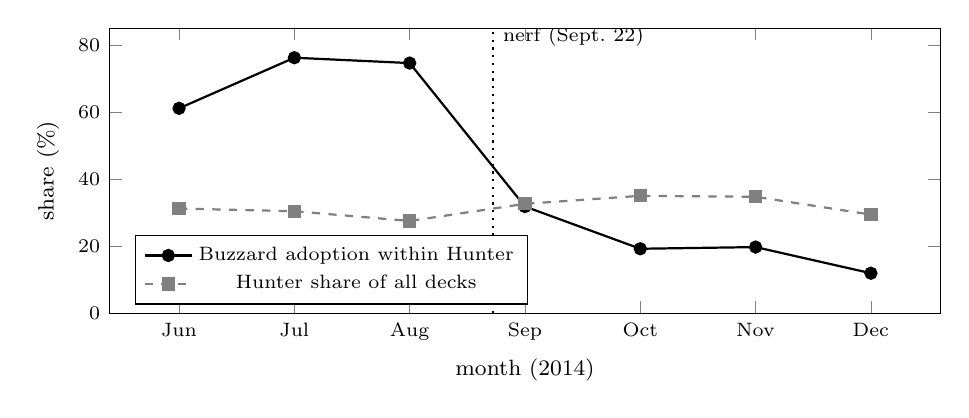
\begin{tikzpicture}
\begin{axis}[
  width=\columnwidth, height=5.2cm,
  xlabel={month (2014)}, ylabel={share (\%)},
  xtick={6,7,8,9,10,11,12},
  xticklabels={Jun,Jul,Aug,Sep,Oct,Nov,Dec},
  ymin=0, ymax=85,
  legend style={font=\scriptsize, at={(0.03,0.03)}, anchor=south west},
  tick label style={font=\scriptsize},
  label style={font=\footnotesize},
  grid=none]
\addplot[mark=*, thick, black] coordinates
  {(6,61.1) (7,76.2) (8,74.6) (9,31.8) (10,19.2) (11,19.7) (12,11.9)};
\addlegendentry{Buzzard adoption within Hunter}
\addplot[mark=square*, dashed, gray, thick, mark options={solid, fill=gray}] coordinates
  {(6,31.2) (7,30.4) (8,27.5) (9,32.6) (10,35.0) (11,34.7) (12,29.4)};
\addlegendentry{Hunter share of all decks}
\draw[dotted, thick] (axis cs:8.72,0) -- (axis cs:8.72,85)
  node[pos=0.97, right, font=\scriptsize] {nerf (Sept.~22)};
\end{axis}
\end{tikzpicture}
\caption{The card--class dissociation. The nerf collapses Buzzard's
within-Hunter adoption while Hunter's class share does not move
outside its noise band.}
\label{fig:dissociation}
\end{figure}

\subsection{Why shocks are the predictable part}
\label{sec:dynamics}
Before predicting shocks we tested the smoother alternative: does an
archetype's field-weighted simulated win rate (its matchup row
weighted by the current popularity mix) predict its next-month
popularity change, in the manner of replicator dynamics? Over 36
(archetype, month) points in the pre-Naxxramas window the Spearman
correlation is $-0.004$, and $0.081$ when the matchup matrix is
re-simulated with the stronger MCTS agent, so the null is not an
artifact of agent choice. The target itself appears to be noise at
this granularity. At $\sim$580 classified decks per month, the
binomial standard error of a share change ($\sim$2.2$\pp$) is
comparable to the observed mean absolute change (2.9$\pp$), and the
lag-1 autocorrelation of changes ($-0.46$) sits at the $-0.5$
expected for a constant series plus independent noise. In a separate
88-deck snapshot, per-deck win rate and play count are uncorrelated
(Spearman $-0.03$). Card adoption around shocks moves by
40--60$\pp$ against that $\sim$2$\pp$ floor. That is where the
signal is, and it is what the rest of the paper predicts.

\section{Prediction Pipeline}
\label{sec:pipeline}

Fig.~\ref{fig:pipeline} summarises the pipeline. All experiments
share the same skeleton: seed with the real pre-shock decks, evolve
under the post-shock card pool (expansion cards added, or nerf
patches applied), extract per-card adoption from the evolved
population, and compare against real post-shock adoption. Deck
fitness is evaluated by simulated matches against a refreshing
field: a gauntlet seeded with real pre-shock representatives of all
three classes and periodically re-sampled from the co-evolving
populations' elites, with a fraction of real anchors retained,
because a fixed gauntlet measurably overfits. Decks are piloted by
the tuned greedy agent with self-play-optimised weights. Every
metric is also computed for the no-change baseline, which predicts
that post-shock adoption equals pre-shock adoption.

\begin{figure}[t]
\centering
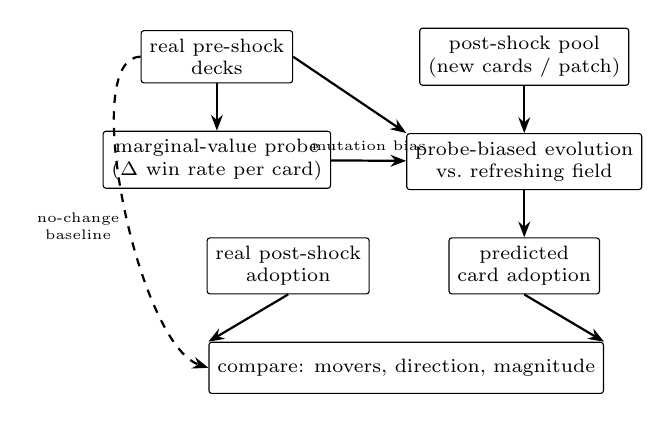
\begin{tikzpicture}[font=\scriptsize,
  box/.style={draw, rounded corners=1pt, align=center, inner sep=3pt,
              minimum height=6.5mm},
  arr/.style={-{Stealth[length=2mm]}, thick}]
\node[box] (seeds) {real pre-shock\\decks};
\node[box, right=16mm of seeds] (pool) {post-shock pool\\(new cards / patch)};
\node[box, below=6mm of seeds] (probe) {marginal-value probe\\($\Delta$ win rate per card)};
\node[box, below=6mm of pool] (evo) {probe-biased evolution\\vs.\ refreshing field};
\node[box, below=6mm of evo] (pred) {predicted\\card adoption};
\node[box, left=10mm of pred] (real) {real post-shock\\adoption};
\node[box, below=6mm of $(real.south)!0.5!(pred.south)$] (cmp)
  {compare: movers, direction, magnitude};
\draw[arr] (seeds) -- (probe);
\draw[arr] (pool) -- (evo);
\draw[arr] (seeds.east) -- (evo.north west);
\draw[arr] (probe) -- node[above, font=\tiny]{mutation bias} (evo);
\draw[arr] (evo) -- (pred);
\draw[arr] (pred.south) -- (cmp.north east);
\draw[arr] (real.south) -- (cmp.north west);
\draw[arr, dashed] (seeds.west) .. controls +(-8mm,0) and +(-9mm,3mm) ..
  node[left, align=center, font=\tiny, pos=0.55]{no-change\\baseline}
  (cmp.west);
\end{tikzpicture}
\caption{Prediction pipeline. Real pre-shock decks seed both the
per-card probe and the evolutionary search; the probe's card values
bias mutation; predictions are scored against real post-shock
adoption alongside a no-change baseline.}
\label{fig:pipeline}
\end{figure}

\subsection{Attempt 1: unbiased evolution fails, with a mechanism}
Real pre-Naxxramas seeds evolving under the Classic+Naxxramas pool
adopted approximately none of the cards the real community adopted.
The cause is drift. A single-card swap changes a deck's win rate by
$\sim$1$\pp$; the per-deck evaluation budget (4--12 games under
early stopping) has a noise floor an order of magnitude above that;
and the observed adoption rate of new cards matches the pure
mutation-drift expectation. Whole-deck fitness evaluation cannot
resolve single-card quality at any budget we could afford, which for
this study was roughly 37{,}000 games.

\subsection{The marginal-value probe}
The probe isolates the card variable directly. For each candidate
card and class, swap the candidate into a fixed slot of five real
host decks, play a fixed 60-game schedule per host against a fixed
nine-deck real field, and record the mean win-rate delta relative to
the unmodified hosts. The result is one number per (card, class):
the card's marginal value in a realistic deck context.

\subsection{Attempt 2: probe-biased evolution}
Real players do not explore a new set uniformly at random. They read
the cards and disproportionately test the ones that look strong. We
model this with a biased mutation operator: probed-positive cards
are proposed more often, and probed-negative slots are replaced more
often, while selection is left untouched (24 fixed games per
evaluation, 25 generations). The claim under test is therefore that
simulation-derived card values combined with evolutionary selection
reproduce the shift. It is not that blind evolution discovers the
shift; the unbiased failure above is reported for exactly that
reason.

\section{Results}
\label{sec:results}

\subsection{The probe recovers the real adoption ranking}
For the Naxxramas launch, the probe's top Hunter cards are the real
community's staple package: Sludge Belcher $+6.5\pp$, Mad Scientist
$+5.3\pp$, Webspinner $+5.1\pp$, Haunted Creeper $+3.7\pp$. All four
reached 45--74\% real adoption within weeks. The cards the community
never played probe at the bottom. Spearman correlation between
probed value and real pre-nerf adoption over the 22 new cards per
class is 0.35 (Hunter), 0.20 (Mage) and 0.30 (Warrior). The two
systematic misses are informative. Death's Bite (probed last for
Warrior, against 60\% real adoption) is a weapon whose value depends
on sequencing its deathrattle across turns. Duplicate ($-3.0\pp$
probed, 41\% real) is a secret whose value is contextual card
advantage. Neither property is visible to a 1-ply evaluator piloting
a single-card swap, and both are instances of the agent-skill
ceiling measured in Sec.~\ref{sec:fidelity}.

\subsection{Expansion: predicting Naxxramas adoption}
Probe-biased evolution from real pre-Naxxramas seeds adopts the real
package. On the 38 Hunter cards whose real adoption moved by at
least 5$\pp$ across the launch, the predicted direction matches
reality for 30, against 16 for unbiased evolution; chance is 19.
Magnitudes land in range for the package cards. Unstable Ghoul is
predicted at 45.8\% against a real 44.9\%, and Mad Scientist,
Undertaker, Sludge Belcher and Loatheb all rise from zero to rates
in the real ordering. Death's Bite stays at 0\% predicted. The
probe's blind spot propagates through the pipeline, as it must.

\subsection{Patch: predicting the nerf response}
The nerf experiment is the cleaner test, since no new cards are
involved and the real post-shock pool equals the simulated pool.
Seeds are real Naxxramas-era decks; the pool applies the real
September patch. Table~\ref{tab:nerf} and Fig.~\ref{fig:nerf} show
the headline cards. The Buzzard collapse is reproduced in direction
and rough magnitude. Nerfed Leeroy drops. Unleash the Hounds, which
the patch left alone, is correctly retained, and Webspinner's
continued rise is called. The removal probe alone already carries
the sign of the response: deleting Buzzard from patched-world Hunter
decks gains $+2.7\pp$, deleting Leeroy $+0.9\pp$ (Hunter) and
$+1.6\pp$ (Warrior).

\begin{table}[t]
\caption{Nerf-response prediction (Hunter, within-class adoption).}
\label{tab:nerf}
\centering
\begin{tabular}{lrrr}
\toprule
card & pre-nerf & predicted & real post-nerf\\
\midrule
Starving Buzzard (nerfed) & 73.4\% & 31.8\% & 16.8\%\\
Leeroy Jenkins (nerfed) & 34.8\% & 4.5\% & 12.0\%\\
Unleash the Hounds & 84.4\% & 77.3\% & 69.5\%\\
Webspinner & 54.4\% & 63.6\% & 73.7\%\\
\bottomrule
\end{tabular}
\end{table}

\begin{figure}[t]
\centering
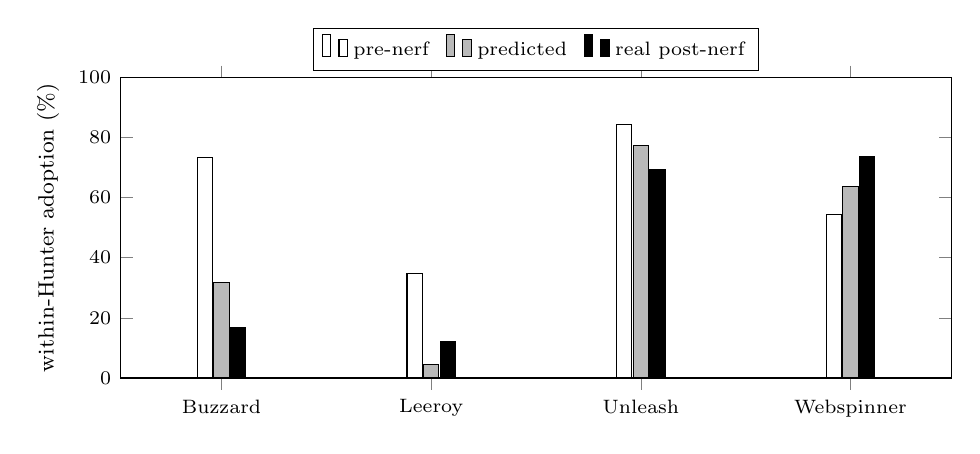
\begin{tikzpicture}
\begin{axis}[
  width=\columnwidth, height=5.4cm,
  ybar, bar width=5.5pt,
  ymin=0, ymax=100, ylabel={within-Hunter adoption (\%)},
  symbolic x coords={Buzzard, Leeroy, Unleash, Webspinner},
  xtick=data,
  enlarge x limits=0.16,
  legend style={font=\scriptsize, at={(0.5,1.02)}, anchor=south,
                legend columns=3, /tikz/every even column/.append style={column sep=4pt}},
  tick label style={font=\scriptsize},
  label style={font=\footnotesize}]
\addplot+[bar shift=-6pt, draw=black, fill=white] coordinates
  {(Buzzard,73.4) (Leeroy,34.8) (Unleash,84.4) (Webspinner,54.4)};
\addlegendentry{pre-nerf}
\addplot+[bar shift=0pt, draw=black, fill=gray!55] coordinates
  {(Buzzard,31.8) (Leeroy,4.5) (Unleash,77.3) (Webspinner,63.6)};
\addlegendentry{predicted}
\addplot+[bar shift=6pt, draw=black, fill=black] coordinates
  {(Buzzard,16.8) (Leeroy,12.0) (Unleash,69.5) (Webspinner,73.7)};
\addlegendentry{real post-nerf}
\end{axis}
\end{tikzpicture}
\caption{Nerf-response prediction against reality. Both nerfed cards
are predicted to fall, the untouched Unleash the Hounds is retained,
and Webspinner's rise is called.}
\label{fig:nerf}
\end{figure}

\subsection{The baseline}
The no-change baseline wins the overall adoption Spearman, at
0.62--0.96 against the prediction's 0.27--0.51. Real decks are
sticky, and a baseline that copies roughly 100 unmoved cards is
unbeatable on a rank metric dominated by non-movers. The
prediction's advantage is confined to the movers, in direction
hit-rate and in the magnitudes above. Since predicting the movers is
the question a no-change baseline cannot answer by construction, we
report both numbers and leave the weighting to the reader.

\section{Learned Evaluators and Unseen Cards}
\label{sec:neural}

The probe's evaluator is a hand-designed linear function, and the
new cards were probed with full knowledge of their implementation. A
stronger test of generalisation replaces it with a learned value
function that has never seen the new cards. Each card is encoded by
68 identity-free mechanical features (cost and stats, type,
keywords, trigger and effect categories, effect magnitudes), so a
nerfed card encodes differently from its original. A small deep-sets
value network of about 60k parameters is trained on pre-Naxxramas
self-play only, with Monte Carlo outcome targets and no search in
the training loop.

Probing the Naxxramas cards with this net splits by mechanism
support. Mage valuations beat the linear probe (Spearman against
real adoption $+0.30$ vs.\ $+0.20$), Warrior ties, and Hunter fails
($-0.075$ vs.\ $+0.35$). The Hunter package consists of
deathrattle-token cards, a mechanism with essentially no support in
pre-Naxxramas training data. Three generations of fine-tuning with
Naxxramas cards in the self-play pool close the gap (Hunter
$-0.075$ to $+0.34$; Mage rises to $+0.60$). The binding constraint
is mechanism coverage of the training distribution, not the
architecture. Given only the patch text, the net assigns the
correct sign to both 2014 nerfs, agreeing with the linear agent on
Buzzard and improving on Leeroy. The two sequencing misses, Death's
Bite and Duplicate, persist under every static evaluator we tested;
they belong to the policy rather than to the evaluation.

\section{Limitations}
\label{sec:limitations}

The probe bias injects simulation-derived knowledge into
exploration, and unbiased evolution fails; we frame the claim
accordingly. Both persistent misses trace to the piloting agent's
1-ply horizon, quantified independently by the fidelity study, so
claims about sequencing-dependent cards are out of reach at this
agent strength. The engine models three classes and one era, and
cross-class effects, such as a nerf pushing players toward an
unmodelled class, are invisible to it. The pre-nerf ground-truth
window may retain a small number of post-nerf-edited decks, because
the September patch received no archive tag of its own; the
window's healthy 73.4\% Buzzard rate bounds that contamination as
minor. Ground-truth matchup win rates are banded at $\pm2.5\pp$,
so we use ordinal ranks where precision matters. Finally, the
evolutionary stages are single runs. The probe aggregates five
hosts and 60 games per card, but replication across seeds remains
future work.

\section{Conclusion}

Given pre-shock decklists and a validated simulator, a
marginal-value probe combined with probe-biased evolutionary
selection predicts which cards a real player population adopted and
abandoned around an expansion and around a nerf. The failure modes
are quantified and localise to agent skill; the no-change baseline
is reported alongside the wins; and a learned evaluator shows the
same predictions emerging from card mechanics alone where training
coverage allows. Forward validation against measured human
adoption, recently established for tier bans~\cite{saravanan2024meta},
strikes us as the appropriate standard for automated balancing
research, and this work extends its coverage to the expansion and
nerf shocks that make up most of a collectible card game's life.

% ------------------------------------------------------------------
\begin{thebibliography}{9}
% All entries verified against the actual publications (2026-08-11):
% titles, authors, venues, years and DOIs checked via publisher pages.

\bibitem{garcia2016evodeck}
P.~Garc\'ia-S\'anchez, A.~Tonda, G.~Squillero, A.~M.~Mora, and
J.~J.~Merelo, ``Evolutionary deckbuilding in Hearthstone,'' in
\emph{Proc. IEEE Conf. Computational Intelligence and Games (CIG)},
2016.

\bibitem{fontaine2019mapelites}
M.~C.~Fontaine, S.~Lee, L.~B.~Soros, F.~de~Mesentier~Silva,
J.~Togelius, and A.~K.~Hoover, ``Mapping Hearthstone deck spaces
through MAP-Elites with sliding boundaries,'' in \emph{Proc. Genetic
and Evolutionary Computation Conf. (GECCO)}, 2019.

\bibitem{dockhorn2019competition}
A.~Dockhorn and S.~Mostaghim, ``Introducing the Hearthstone-AI
competition,'' \emph{arXiv preprint arXiv:1906.04238}, 2019.

\bibitem{swiechowski2018}
M.~\'Swiechowski, T.~Tajmajer, and A.~Janusz, ``Improving Hearthstone
AI by combining MCTS and supervised learning algorithms,'' in
\emph{Proc. IEEE Conf. Computational Intelligence and Games (CIG)},
2018.

\bibitem{demesentier2019meta}
F.~de~Mesentier~Silva, R.~Canaan, S.~Lee, M.~C.~Fontaine,
J.~Togelius, and A.~K.~Hoover, ``Evolving the Hearthstone meta,'' in
\emph{Proc. IEEE Conf. on Games (CoG)}, 2019.

\bibitem{saravanan2024meta}
A.~Saravanan and M.~Guzdial, ``A framework for predicting the impact
of game balance changes through meta discovery,'' \emph{IEEE Trans.
Games}, 2024, arXiv:2409.07340.

\bibitem{justesen2017}
N.~Justesen, T.~Mahlmann, S.~Risi, and J.~Togelius, ``Playing
multiaction adversarial games: Online evolutionary planning versus
tree search,'' \emph{IEEE Trans. Games}, vol.~10, no.~3, pp.~281--291,
2018, doi:10.1109/TCIAIG.2017.2738156.

\bibitem{dockhorn2018prediction}
A.~Dockhorn, M.~Frick, \"U.~Akkaya, and R.~Kruse, ``Predicting
opponent moves for improving Hearthstone AI,'' in \emph{Proc. Int.
Conf. Information Processing and Management of Uncertainty (IPMU)},
Springer, 2018, pp.~621--632, doi:10.1007/978-3-319-91476-3\_51.

\bibitem{zenodo_dataset}
P.~Garc\'ia-S\'anchez, A.~Tonda, A.~Fern\'andez-Ares, and A.~Mora,
``Hearthstone Decks Dataset,'' Zenodo, v1, 2023,
doi:10.5281/zenodo.10198504.

\bibitem{vicious_syndicate}
Vicious Syndicate, ``Data Reaper Report: Classic,'' 2021. [Online].
Available: \url{https://www.vicioussyndicate.com}

\bibitem{hansen2001cmaes}
N.~Hansen and A.~Ostermeier, ``Completely derandomized
self-adaptation in evolution strategies,'' \emph{Evolutionary
Computation}, vol.~9, no.~2, pp.~159--195, 2001.

\bibitem{mouret2015mapelites}
J.-B.~Mouret and J.~Clune, ``Illuminating search spaces by mapping
elites,'' \emph{arXiv preprint arXiv:1504.04909}, 2015.

\end{thebibliography}

\end{document}
